\section{Uvod}

Tema ovog projekta je razvijanje globalnog informacionog sistema za Medj{}ugradski autobuski prevoz u nasoj zemlji. Rad je radj{}en kao projekat iz predmeta "Informacioni sistemi" na Matemati\v ckom fakultetu. Informacioni sistem bi trebao da olak\v sa probleme pri kupovini i rezervaciji karata. Omogu\'cava nam da bez odlaska na samu stanicu izvr\v simo rezervaciju karte kao i rezervaciju mesta ili eventualnu reklamaciju. Zaposlenima na autobuskoj stanici pru\v za uvid u slobodan broj mesta i olak\v sava prodaju karata.
\section {Analiza sistema}

Ovaj informacioni sistem nam pru\v za mogu\'cnost da izaberemo po\v cetnu i krajnju stanicu, kao i datum polaska. Sistem nam daje uvid u sve polaske za datu destinaciju na odabrani datum kao i cene karata. 
Osnovna namena na\v seg informacionog sistema je da na \v sto efikasniji na\v cin omogu\'ci kupovinu/prodaju, rezervaciju (kako karata tako i mesta) i eventualne reklamacije. Kupovina je mogu\'ca iskljucivo na \v salteru, dok se rezervacija i reklamacija mogu obaviti putem telefona ili online. Ukoliko se kupac koji je rezervisao kartu ili mesto ne pojavi do odredjenog vremena, rezervacija se ponistava. Prilikom kupovine kupac ostvaruje pravo na neke od popusta omogu\'cene od strane prevoznika. Da bi se to \v sto efikasnije izvelo sistem mora da brine i o raspolo\v zivim resursima na polaznoj stanici. Svakog trenutka sistem mora da ima uvid o broju raspolo\v zivih mesta na izabranoj pocetnoj stanici (koliko je putnika u\v slo i iza\v slo na predhodnim stanicama). U slu\v caju velikog interesovanja (do nekog odredjenog perioda, 5 min pre dolaska autobusa na peron) sistem obave\v stava da \'ce biti potreban dodatni broj mesta. Ukoliko je prevoznik u mogu\'cnosti (na raspolaganju u blizini ima dodatna vozila i voza\v ce) pove\'cava se broj mesta (trenutni autobus se zamenjuje autobusom sa ve\'cim brojem mesta ili uvodjenjem dodatnog vozila). Takodje, ako je zanteresovanost jako mala, moze se planirani autobus zameniti vozilom manjeg kapaciteta. Sistem vodi racuna i o broju slobodnih perona, da bi u slu\v caju uvodjenja novog vozila ono imalo gde da se smesti (po\v zeljno je da u svakom trenutku imamo slobodan peron). Na jednom peronu razmak izmedju dva polaska treba da bude najmanje 15 minuta.

\section{Dijagram toka podataka}
\begin{figure}[!htb]
	\centering
	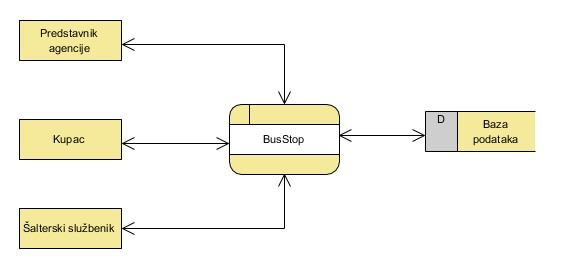
\includegraphics[width=0.7\linewidth]{DTP}
	\caption{Dijagram toka podataka}
	\label{fig:dtp}
\end{figure}



\section{Akteri}
\subsection{Kupac}
\begin{itemize}
	\item Kupuje kartu
	\item Rezervi\v se kartu
	\item Rezervi\v se mesto
	\item Reklamira kartu
\end{itemize}
\subsection{\v Salterski slu\v zbenik}
\begin{itemize}
	\item Prodaje kartu
	\item Ukoliko je rezervacija ili reklamacija izvr\v sena putem telefona unosi podatke u sistem
\end{itemize}
\subsection{Predstavnik agencije}
\begin{itemize}
	\item Obezbedj{}uje potrebna vozila i voza\v ce
\end{itemize}

\newpage
\section{Slu\v cajevi upotrebe}
\subsection{Online rezervacija karte}
\begin{description}
	\item [$\ast$ Kratak opis: ] Putem veb stranice na\v seg informacionog sistema, kupac mo\v ze dobiti sve potrebne informacije koje se odnose na red vo\v znje, dostupne prevoznike, kao i preciznije detalje o nekoj odredj{}enoj ruti vo\v znje.
	
	\item[$\ast$ U\v cesnici: ] Kupac.
	\item[$\ast$ Preduslovi: ] Pristup internetu.
	\item[$\ast$ Postuslovi: ] Rezervacija karte uspe\v sno poslata u sistem.
	\item[$\ast$ Osnovni tok: ] \ \\
	\renewcommand{\labelenumii}{\Roman{enumii}}
	\begin{enumerate}
		\item Kupac pristupa online sajtu autobuske stanice.
		\item Informi\v se se o dostupnim terminima i redovima vo\v znje za datum i vreme koji mu odgovaraju.
		\item Popunjava formu za rezervaciju karte na kojoj se nalaze detalji poput datuma i vremena polaska.
		\item Sistem vr\v si proveru da li su uneti podaci validni.
		\item Rezervacija karte se pamti u sistem.
		\item Sistem izbacuje poruku kojom obave\v stava kupca o uspe\v snoj ili neuspe\v snoj prijavi.
	\end{enumerate}
	\item[$\ast$ Alternativni tok: ]
	\begin{enumerate}
		\item[4a. ] Ukoliko podaci sa forme za rezervaciju karte nisu korektni sistem odgovaraju\v com porukom obave\v stava kupca i stranica na kojoj se nalazi forma se oslve\v zava
	\end{enumerate}
	
\end{description}
\newpage
\subsection{Kupovina karte}
\subsubsection{Kupovina ako karta nije unapred rezervisana}
\begin{description}
	\item[$\ast$ Kratak opis: ] Kupac na \v salteru kupuje kartu za \v zeljenu destinaciju. Slu\v zbenik na \v salteru unosi podatke u sistem i \v stampa kartu ukoliko ima slobodnog mesta u autobusu.
	\item[$\ast$ U\v cesnici: ] Kupac i slu\v zbenik na \v salteru.
	\item[$\ast$ Preduslovi: ] Kupac dolazi na stanicu.
	\item[$\ast$ Tok: ] \ \\
	\begin{enumerate}
		\item Kupac dolazi na \v salter.
		\item Zatra\v zi informacije o vremenima polazaka, prevoznicima i cenama karte ukoliko to vec nije u\v cinio.
		\item Slu\v zbenik na \v salteru mu daje \v zeljene informacije
		\item Kupac se izja\v snjava za vreme polaska i \v zeljenog prevoznika (ukoliko vi\v se prevoznika polazi u isto vreme).
		\item Slu\v zbenik unosi date podatke u sistem.
		\item Sistem proverava da li ima slobodnog mesta u tom terminu.
		\item Ukoliko nema slobodnog mesta, a vozilo jo\v s uvek nije postavljeno na peron, sistem proverava da li dati prevoznik ima resurse da zameni teku\'ce vozilo vozilom ve\'ceg kapaciteta ili da uvede dodatno vozilo.
		\item Ukoliko nema mesta i prevoznik nema odgovaraju\'ce dodatne resurse, sistem daje obave\v stenje da nema mesta, a zatim slu\v zbenik to saop\v stava kupcu i kupovina se smatra neuspe\v snom.
		\item Ukoliko ima slobodnog mesta ili prevoznik na raspolaganju ima potrebne resurse, sistem daje obave\v stenje da je kupovinu mogu\'ce izvr\v siti.
		\item Slu\v zbenik saop\v stava kupcu da ima mesta u autobusu.
		\item Kupac potvrdjuje da \v zeli da kupi kartu i nagla\v sava da li \v zeli kartu u jednom smeru ili povratnu.
		\item Ukoliko kupac ima pravo na neki od popusta, saop\v stava to slu\v zbeniku i pokazuje odgovaraju\'ca dokumenta kao dokaz.
		\item Slu\v zbenik unosi podatke o popustu i podatke da li je karta povratna ili u jednom smeru.
		\item Sistem \v stampa kartu.
		\item Kupac pla\' ca kartu.
		\item Slu\v zbenik uzima novac i daje kartu kupcu tako da se kupovina smatra uspe\v snom.
	\end{enumerate}
\end{description}

\subsection{Reklamacija}

\begin{description}
  \item[$\ast$ Kratak opis: ] Kupac mo\v ze reklamirati kupljenu kartu na \v salteru. Ukoliko nije prekasno, slu\v zbenik na \v salteru preuzima kartu i osloba\dj a mesto u sistemu i zatim vraca novac korisniku.
  \item[$\ast$ U\v cesnici: ] Kupac i slu\v zbenik na \v salteru
  \item[$\ast$ Preduslovi: ] Kupac ima va\v ze\'cu kartu i do polaska autobusa ima barem sat vremena
  \item[$\ast$ Postuslovi: ] Kupac je vratio kartu i dobio novac natrag
  \item[$\ast$ Osnovni tok: ] \ \\
  \begin{enumerate}
    \item Kupac dolazi na \v salter i obave\v stava slu\v zbenika o nameri da vrati kartu
    \item Slu\v zbenik proverava da li su ispunjeni uslovi za reklamaciju
    \item Ukoliko su uslovi ispunjeni, slu\v zbenik preuzima kartu
    \item Slu\v zbenik poni\v stava kartu i osloba\dj a mesto u sistemu
    \item Slu\v zbenik vra\'ca novac kupcu
  \end{enumerate}
  \item[$\ast$ Alternativni tok]
  \begin{enumerate}
    \item[3a. ]  Ukoliko uslovi nisu ispunjeni, slu\v zbenik obavestava kupca
  \end{enumerate}
  
\end{description}

